\documentclass[a4paper, 11pt]{article}

\usepackage{graphicx}
\usepackage{graphics}
\usepackage{verbatim}
\usepackage{listings}
\usepackage{color}

\begin{document}

\title{IGREBOOT bootloader}
\author{IGREBOT team}
\date{}

\maketitle


\newpage
\tableofcontents
\addtocontents{toc}{\protect\setcounter{tocdepth}{1}}


\newpage
\begin{abstract}
This document describes the IGREBOOT related softwares.
\end{abstract}


\newpage
\section{Introduction}

\subsection{Overview}
\paragraph{}
To ease software management on the 2012 robot, the different electronic board
microcontrollers are flashed with a bootloader. The bootloader is in charge
of updating the board software on demand. This is done from a host PC software.
The commands are carried over CAN. Since PCs usually do not have CAN interfaces,
a serial to CAN bridge is implemented.

\begin{figure}[]
\centering
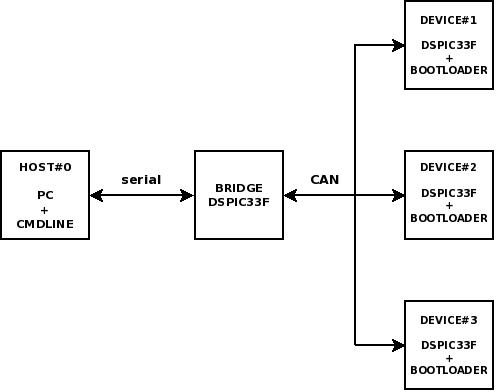
\includegraphics[scale=0.5]{./dia/global_view/main.jpeg}
\caption{global view}
\label{global_view}
\end{figure}

\paragraph{}
The project source code is temporarly maintained in a GIT repository:
\begin{center}
https://github.com/texane/igreloader
\end{center}

\paragraph{}
The project depends on the following softwares:
\begin{itemize}
\item a working LINUX system with standard GNU tools,
\item MPLABX version 1.0 .
\end{itemize}
Note that WINDOWS and MACOSX are not yet supported.

\paragraph{}
The project tree is organized as follow:
\begin{itemize}
\item src/blinker
\item src/bridge
\item src/device
\item src/host
\end{itemize}

\newpage
\section{Bootloader}
\paragraph{}
The bootloader waits for commands targeted at the specified device. The following commands are implemented:
\begin{itemize}
\item CMD\_ID\_WRITE\_PMEM
\item CMD\_ID\_READ\_PMEM
\item CMD\_ID\_WRITE\_CMEM
\item CMD\_ID\_STATUS
\item CMD\_ID\_GOTO
\end{itemize}

\paragraph{}
Figure \ref{memory_map} shows the memory organization for a DSPIC33F128GP802 microcontroller. Refer
to the reference manual, figure 4-1 for more information.
\paragraph{}
The red areas are reserved for the bootloader and should not be used by the user application. To prevent
the application from using reserved areas, a modified linker script can be used. Such a linker script can
be found in:
\begin{center}
igreloader/build/blinker.X/igreboot\_p33FJ128GP802.gld
\end{center}

\begin{figure}[]
\centering
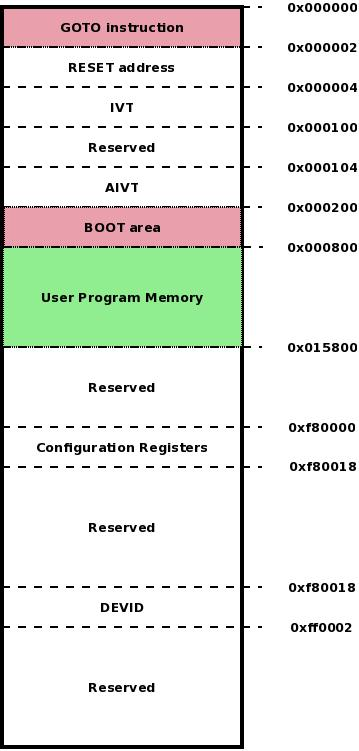
\includegraphics[scale=0.4]{./dia/memory_map/main.jpeg}
\caption{memory map}
\label{memory_map}
\end{figure}


\newpage
\section{Host PC software}
\paragraph{}
TODO: command line

\paragraph{}
The following listing contains the commands used in a typical session:
\begin{tiny}
\begin{lstlisting}[frame=tb]

# go to the project source tree
texane@dell:~$ cd /home/texane/repo/igreloader/

# compile a sample application
texane@dell:~/repo/igreloader$ cd build/blinker.X/
texane@dell:~/repo/igreloader/build/blinker.X$ make

# return to build directory and compile the host software. Omit if already done.
texane@dell:~/repo/igreloader/build/blinker.X$ cd ..
texane@dell:~/repo/igreloader/build$ ./do_build_host.sh

# write the application to device flash
./a.out write /dev/ttyUSB0 2 ./blinker.X/dist/default/production/blinker.X.production.hex noconf

# order the device to execute the application
texane@dell:~/repo/igreloader/build$ ./a.out goto /dev/ttyUSB0 2 800
\end{lstlisting}
\end{tiny}


\newpage
\section{Serial to CAN Bridge}
\paragraph{}
As PCs usually do not have a CAN interface, a serial to CAN bridge has been implemented. Its purpose is to
wrap CAN payloads plus minimal meta information into a serial frame. The wrapping format is described in
Figure XXX.


\newpage
\section{Sample applications}
\paragraph{}
TODO: blinker


\newpage
\section{TODOS}
\paragraph{}
\begin{itemize}
\item bootloader linker map from 0x200 to 0x800
\item add CAN support to bootloader
\item implement serial to CAN brigde
\end{itemize}


\end{document}
